
%%%%%%%%%%%%%%%%%%%%%%% file typeinst.tex %%%%%%%%%%%%%%%%%%%%%%%%%
%
% This is the LaTeX source for the instructions to authors using
% the LaTeX document class 'llncs.cls' for contributions to
% the Lecture Notes in Computer Sciences series.
% http://www.springer.com/lncs       Springer Heidelberg 2006/05/04
%
% It may be used as a template for your own input - copy it
% to a new file with a new name and use it as the basis
% for your article.
%
% NB: the document class 'llncs' has its own and detailed documentation, see
% ftp://ftp.springer.de/data/pubftp/pub/tex/latex/llncs/latex2e/llncsdoc.pdf
%
%%%%%%%%%%%%%%%%%%%%%%%%%%%%%%%%%%%%%%%%%%%%%%%%%%%%%%%%%%%%%%%%%%%


\documentclass[runningheads,a4paper]{llncs}
%\linespread{2.5}
\usepackage{amssymb}
\setcounter{tocdepth}{3}
\usepackage{graphicx}
\usepackage{algorithm}
\usepackage[noend]{algpseudocode}
\renewcommand{\algorithmicrequire}{\textbf{Input:}}
\renewcommand{\algorithmicensure}{\textbf{Output:}}

\usepackage{url}
\newcommand{\keywords}[1]{\par\addvspace\baselineskip
\noindent\keywordname\enspace\ignorespaces#1}

\newcommand{\includegraphicsfit}[1]
{\includegraphics[width=\columnwidth,height=\textheight,keepaspectratio]{#1}}

\newcommand{\BigO}[1]{$\mathcal{O}{(#1)}$}

% Fancy proofs
\let\proof\relax
\let\endproof\relax
\usepackage{amsthm}

\begin{document}

\mainmatter  % start of an individual contribution

% first the title is needed
\title{Hyperplane Elimination for Quickly Enumerating Local Optima}

% a short form should be given in case it is too long for the running head
%\titlerunning{Lecture Notes in Computer Science: Authors' Instructions}

% the name(s) of the author(s) follow(s) next
%
% NB: Chinese authors should write their first names(s) in front of
% their surnames. This ensures that the names appear correctly in
% the running heads and the author index.
%
%\author{Brian W.~Goldman\and William F. Punch}
\author{Anonymous Author\and Anonymous Author}

%
%\authorrunning{Lecture Notes in Computer Science: Authors' Instructions}
% (feature abused for this document to repeat the title also on left hand pages)

% the affiliations are given next; don't give your e-mail address
% unless you accept that it will be published
%\institute{BEACON Center for the Study of Evolution in Action,\\
%Michigan State University, U.S.A.\\
%brianwgoldman@acm.org, punch@msu.edu}
\institute{Department\\ Organization\\ Email}

%
% NB: a more complex sample for affiliations and the mapping to the
% corresponding authors can be found in the file "llncs.dem"
% (search for the string "\mainmatter" where a contribution starts).
% "llncs.dem" accompanies the document class "llncs.cls".
%

%\toctitle{Lecture Notes in Computer Science}
%\tocauthor{Authors' Instructions}
\maketitle


\begin{abstract}
Examining the properties of local optima is a common method for understanding
combinatorial-problem landscapes.
Unfortunately,
exhaustive methods for finding local optima are limited to very small problem sizes.
We propose a method for exploiting problem structure
to skip hyperplanes
that cannot contain local optima, allowing runtime to scale with
the number of local optima instead of with the landscape size.
We prove optimality for linear and $k$-bounded separable problems, and we provide
empirical evidence of optimality on NKq Landscapes and Ising Spin Glasses.
We further refine this method to find only solutions
that cannot be improved by flipping $r$ or fewer bits, which counterintuitively
can reduce total runtime. While previous methods were limited to
landscapes with at most $2^{34}$ binary strings, hyperplane elimination can enumerate the same problems with
$2^{77}$ binary strings, and find all 4-bit local optima to problems with $2^{200}$ binary strings.
We believe this increase in size will help further our understanding of complex real-world landscapes.



%The abstract should summarize the contents of the paper and should
%contain at least 70 and at most 150 words. It should be written using the
%\emph{abstract} environment.
\keywords{Landscape Understanding, Gray-Box, Mk Landscapes}
\end{abstract}


\section{Introduction}
The ruggedness and high dimensionality of most problem landscapes makes them challenging to
analyze and understand. However, doing so can be helpful in
quantifying the difficulty of a problem. Furthermore,
this information can be used to design search algorithms that specifically deal
with those difficulties. 
Similarly, knowing problem characteristics that favor
a particular
algorithm can help researchers choose the algorithm
most likely to perform well on their problem.

A common way of analyzing landscapes is to
examine both the frequency and distribution of local optima~\cite{boese:1994:bigvalley},
as well as how different search operators transition between these
optima~\cite{tomassini:2008:nknetworks,verel:2011:nknetworks,ochoa:2015:crossovernetworks}.
However, finding all of the local optima of a complex problem is prohibitively time consuming
even for small problems. Many studies have been limited to 18-bit
problems~\cite{tomassini:2008:nknetworks,verel:2011:nknetworks} due to this time constraint.
By leveraging recent advancements in Gray-Box optimization that allow for
constant time local search~\cite{chicano:2014:ball}, this limit was raised
to 30-bit problems~\cite{ochoa:2015:crossovernetworks}. While sampling
methods can approximate some of these statistics for much larger
landscapes~\cite{iclanzan:2014:somnetworks}, they do not provide enough
detail necessary for some metrics~\cite{ochoa:2015:crossovernetworks}.

Here we introduce a method for finding all local optima for the same problems using
up to 77 bits. The cornerstone of this method is the identification
of hyperplanes that cannot contain any local optima, allowing large
portions of the search space to be skipped during enumeration.
The techniques developed here can be applied to the generalized problem class of Mk Landscapes,
which contains many real world and benchmark combinatorial problems.



\section{Mk Landscapes as a tool for Problem Generalization}
\label{sec-mk}
An Mk Landscape~\cite{whitley:2015:mk} is any function
who's value is equal to the sum of a set of subfunctions.
Each subfunction uses a small subset of variables from the original function's input.
Combined with limits on the number of subfunctions and the size of each subfunction's
subset, Mk Landscapes can be efficiently searched for both local~\cite{whitley:2012:constant,chicano:2014:ball}
and global~\cite{goldman:2015:GBO,tintos:2015:partitioncross} optima.

Formally, an Mk Landscape is any function $f : \mathbb{B}^{N}\rightarrow \mathbb{R}$
that can be expressed in the following form:
\begin{equation}
  f(x) = \sum_{i=1}^{M} f_i(mask(x, s_i))
  \label{eq-mk}
\end{equation}
In this equation $f_i$ is a subfunction such that $f_i : \mathbb{B}^{|s_i|}\rightarrow \mathbb{R}$.
Each $s_i$ is a set of variables in $x$, such that $|s_i| \leq k$.
The $mask$ function
returns the values in $x$ associated with each variable in $s_i$.
The total number of subfunctions $M$ is constrained to grow at \BigO{N}, and $k$
is constant with respect to $N$.

This formulation can represent many problems of real-world interest, as well as
the most commonly used combinatorial benchmark problems. In this work we
examine 5 problems in particular: Concatenated Traps, Adjacent and Random NKq Landscapes,
Ising Spin Glasses, and MAX-kSAT.

The Concatenated Trap problem~\cite{deb:1992:trap} is a composition of $k$-order deceptive,
separable subfunctions. In Mk Landscape terms, $M=N/k$ such that $\forall_i |s_i| = k$ and
$\forall_{i \neq j} s_i \cap s_j = \emptyset$. Each $f_i$ applies an identical subfunction based
on the number of variables set to 1:
\begin{equation}
   trap(t) = \left\{
     \begin{array}{rl}
       k-1-t,~ &  t<k\\
       k,~   &  t = k
     \end{array}
   \right.
  \label{eq-trap}
\end{equation}
While this problem is still in common use~\cite{hsu:2015:dsmgaII,inoue:2015:adaptivep3},
most advanced methods can solve it trivially~\cite{goldman:2012:ltga} and when expressed
as an Mk Landscape it can be solved exactly in \BigO{N} time~\cite{whitley:2015:mk}.
We therefore include it only because its structure allows for straight forward algorithm analysis.
Here we set $k=5$.

NKq landscapes specify a class of randomly generated problem instances using 3 paramters:
(1) the number of problem variables $N$ (2) the amount of variable epistasis $K$ where $k=K+1$
and (3) the number of unique fitness values $q$. From these parameters a landscape is generated
by creating $M=N$ subfunctions $f_i$, where $f_i$ uses variable $x_i$ and $K$ others to look up
a fitness value in the range $[0..q-1]$ from a randomly generated table. This structure
makes NKq landscapes a natural fit for Mk landscapes (sum of bounded subfunctions)
and are the most studied problem class for Gray-Box
optimization~\cite{whitley:2012:constant,chicano:2014:ball,goldman:2015:GBO,tintos:2015:partitioncross,ochoa:2015:crossovernetworks,whitley:2015:mk}.
Here we choose $k=3$ with $q=2^{K+1}=2^{k}=8$.

We use two common variants of NKq in our experiments which specify how the $K$ additional
variables in each subfunction are chosen: Adjacent and Random. In Adjacent NKq, $f_i$ depends
on variable indices $[i..(i+k) \bmod N]$. In Random NKq, $f_i$ depends on $x_i$ and a random
set of $K$ unique variables that does not include $x_i$. While Random NKq is NP-Hard,
the structure of Adjacent NKq allows for a polynomial time dynamic programming solution~\cite{wright:2000:solvingnk}.
Adjacent NKq is therefore often used to approximate a search algorithm's ability to
solve Random NKq.

Ising Spin Glasses are a type of MAX-CUT problem derived from statistical physics.
Each atom in the glass (vertex) can be assigned a spin, with the goal being to
find the set of assignments that minimize the energy between nearby atoms (edges).
Similar to Adjacent NKq, the $2D\pm J$ subset of Ising Spin Glasses can be polynomially
solved~\cite{saul:1994:spinglass}.
In this subset, the graph is defined as a square two-dimensional grid with
periodic boundaries such that each edge
weight is chosen from $\{-1, 1\}$. Each vertex is assigned a spin from $\{-1, 1\}$ with
the energy in the glass equal to
\begin{equation}
\sum_{e_{ij} \in E} x_ie_{ij}x_j
  \label{eq-ising}
\end{equation}
where $e_{ij}$ is the weight of the edge connecting vertex $i$ to vertex $j$. In Mk landscape terms
this type of spin glass has $M=2N$ and $k=2$.

Our final problem is randomly generated maximum satisfiability or MAX-kSAT.
This version of the canonical NP-Complete boolean satisfiability problem is formulated
as the maximization of $M=4.27N$ clauses, each containing exactly $k=3$ unique literals.
A clause is satisfied if any of its literals match how a solution's variables are set.

\section{Gray-Box Enumeration of Mk Landscapes}
\label{sec-gray-box}
When considered as a black box, the process of finding all local optima
in a landscape requires $\Omega(N2^N)$ time. This is because each
of the $2^N$ solutions must be compared with each of its $N$ neighbors.
Extending this method to look for solutions that cannot be improved by
flipping $r$ or fewer bits requires $\Omega(N^r2^N)$ time. However,
by exploiting Gray-Box optimization methods, previous work~\cite{ochoa:2015:crossovernetworks}
was able to find all $r$-bit local optima of Mk Landscapes in \BigO{2^N} for any small,
fixed value of $r$.

The first major result in Gray-Box optimization was the proof that the list
of fitness-improving moves from a solution can be updated after a bit flip in \BigO{1}
time~\cite{whitley:2012:constant}.
The fitness effect of flipping $x_j$ only changes after flipping $x_i$ if
there is a non-linear relationship between $x_i$ and $x_j$.
In an Mk Landscape, variables
can only have a non-linear relationship if they appear together in at least one $s_i$.
Therefore by definition the total number of non-linear
relationships in an Mk Landscape is linear with $N$, meaning on average the amortized
number of non-linear relationships per variable is \BigO{1}.

This result was extended, with no increase in asymptotic costs,
to include search for
solutions that cannot be improved by flipping $r$ or fewer bits~\cite{chicano:2014:ball}.
Consider two variables $x_i$ and $x_j$ that do not appear in the same $s_i$.
By definition the fitness effect of flipping both $x_i$ and $x_j$ is equal to the sum
of flipping each independently. As a result, if neither individual flip is fitness improving,
flipping both together cannot be fitness improving. By examining the graph of non-linear
interactions between variables, this principle can be extended to any collection of $r$
variables, with the number of useful collections growing at \BigO{N} when $r$ is a small constant.
As a result, the time to update the list of improving moves after up to $r$ bit-flips is still \BigO{1}.

These advances can be applied directly to the task of finding all local optima in a
landscape~\cite{ochoa:2015:crossovernetworks}.
Instead of requiring \BigO{N} time to evaluate each solution and to check if it
is a local optima, only \BigO{1} time is needed. Consider an enumeration of the landscape
that uses gray-codes, meaning that each transition between solutions requires exactly 1 bit flip.
In Gray-Box optimization updating fitness and the list of improving moves after a single bit flip
takes \BigO{1} time. That property holds even when looking for $r$-bit fitness-improving moves.
Therefore Gray-Box enumeration is able to find all local optima in \BigO{2^N} time.

\section{Hyperplane Elimination}
\begin{figure}
  \centering
  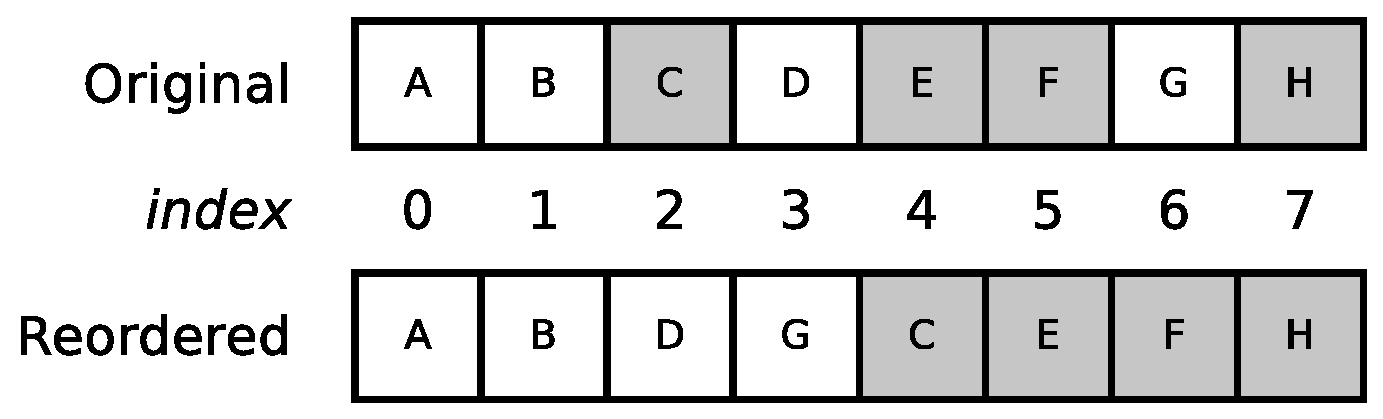
\includegraphics[width=.75\columnwidth,height=\textheight,keepaspectratio]{Enumerate}
  %\includegraphicsfit{Enumerate}
  \caption{Example change of ordering. The gray variables represent all dependencies
           for move $m_i$ which flips variable $F$. By reordering, $m_i$'s lowest $index$ dependency improves from 2 to 4.}
  \label{fig-enumerate}
\end{figure}

Due to the limited non-linearity of the Gray-Box domain, it is possible to exclude large
parts of the search space without missing any local optima.
Consider the representation presented in the top of Figure~\ref{fig-enumerate}. In a Black-Box
domain, enumeration would progress as a binary counter, treating $index$ 0 (symbol $A$ in the solution) as
the least significant bit. This ordering ensures that before changing $index$ $i$, all possible settings of $index$
0 through $i-1$ have been tested. This corresponds to examining the hyperplane where the lowest $i-1$ positions
can vary and all other positions remain fixed. The Gray-Box domain makes it possible to skip hyperplanes
that cannot contain local optima. In Figure~\ref{fig-enumerate}, move $m_i$ which flips variable $F$ is a fitness improvement
when enumeration starts (all variables set to 0). Due to the known relationships between variables,
we know that the quality of $m_i$ only depends on variables $C$, $E$, $F$, and $H$.
Therefore, until one of those four variables are modified, the solution cannot be a local optimum.
As a result, the hyperplane **0*00*0 cannot contain a local optima and can
therefore be eliminated from consideration during enumeration.
More generally, if at any point during enumeration
there exists a fitness-improving move, no local optima can exist until at least one
dependency of that move is modified. Any hyperplane that has all of a fitness-improving
move's dependencies fixed cannot contain any local optima.

\begin{algorithm}
  \caption{Find all local optima using Hyperplane Elimination.}
  \label{alg-enumerate}
  \begin{algorithmic}[1]
    \Require $solution \leftarrow \{0\}^N$
    \Require $move\_bin$ (How many improving moves have each minimum dependency)
    \Require \textproc{MakeMove} (Function that flips $index$ in $solution$ and updates $move\_bin$)
    \Ensure $found$ (list of all local optima)
    \State $found \leftarrow [~]$
    \State $index \leftarrow N-1$
    \While{$index < N$}
      \While{$index > 0$ \textbf{and} $move\_bin[index] = 0$}\label{alg-enumerate-bincheck}
        \State $index \leftarrow index-1$
      \EndWhile
      \If{$index = -1$}
        \State $found \leftarrow found + [solution]$
        \State $index \leftarrow 0$
      \EndIf
      \While{$index < N$ \textbf{and} $solution[index] = 1$}\label{alg-enumerate-counter}
        \State \Call{MakeMove}{$index$}
        \State $index \leftarrow index + 1$
      \EndWhile
      \If{$index < N$}
        \State \Call{MakeMove}{$index$}\label{alg-enumerate-insert}
      \EndIf
    \EndWhile
  \end{algorithmic}
\end{algorithm}

This knowledge can be exploited to skip parts of the enumeration,
as shown in Algorithm~\ref{alg-enumerate}.
Initially all variables are set to 0 and
each fitness-improving move is put into a table $move\_bin$
based on that move's lowest $index$ dependency. This is the first $index$ that
can be modified by enumeration that can potentially change the fitness effect of making that move.
In order to determine how much of the enumeration can be skipped, we must find
the highest $index$ in $move\_bin$ that contains a fitness-improving move,
as done by Line~\ref{alg-enumerate-bincheck}. If no move is fitness-improving,
then a local optimum has been found.

Algorithm~\ref{alg-enumerate} works by finding the highest $index$ in $move\_bin$
that is not empty and then adding a 1 to that $index$ in $solution$. Initially
all bins could contain a fitness-improving move, so $index$ starts at $N-1$.
If at any point all bins are empty then the solution is added to the list of
local optima $found$. Algorithm~\ref{alg-enumerate} then
adds a 1 to $index$ using the loop on Line~\ref{alg-enumerate-counter}
to perform carry operations and Line~\ref{alg-enumerate-insert} to create the new 1 value.
Iteration stops when the carry exceeds the solution length.

When performing subsequent iterations, not all bins need to be checked. Instead, the highest $index$
bin that must be tested is the highest $index$ flipped by the previous iteration. This
simplification is possible because
the previous iterations have verified that all moves in higher $index$ bins are not fitness improving, and no action performed during
that iteration can make them fitness improving.
Furthermore, $index$ is always the location of the least significant 1 bit in $solution$, meaning
iteration can continue immediately from the found $index$. This is true by construction.
Initially $solution$ contains all 0s. Each time a 1 is inserted its position is equal to $index$ and
$index$ is only increased by carry operations which reset a position to 0 before increasing $index$.

Extending Algorithm~\ref{alg-enumerate} to search for $r$-bit optima only requires adding the
necessary $r$-bit moves to $move\_bin$. As discussed in Section~\ref{sec-gray-box}, we know the number of these moves
is \BigO{N} an can be kept updated in \BigO{1} time per flip. Therefore, for small $r$, the cost
of finding $r$-bit local optima is no more than a constant slower than finding 1-bit local optima.
In fact, we will provide evidence in Section~\ref{sec-r-bit} that increasing $r$ can actually
decrease runtime.

\section{Reordering Variables}
\label{sec-reorder}
As a final efficiency, the order in which variables in $solution$ are $index$ed can be reordered.
When a move is fitness-improving,
the amount of search space that is skipped depends on how high its lowest $index$ dependency is. Therefore,
by rearranging the order to make its lowest $index$ dependency higher, more search space can be skipped. 
Figure~\ref{fig-enumerate} shows how changing the $index$ order of variables
improves $m_i$'s lowest $index$ dependency from 2 to 4. Consider that before reordering $m_i$ allows the hyperplane
**000000 to be skipped by Algorithm~\ref{alg-enumerate}, while after reordering the hyperplane that can be skipped is ****0000.
Now, whenever $m_i$ is a fitness improvement, 4 times as many solutions are skipped.

We perform this reordering in a greedy fashion, such that the move with the
least-unmapped dependencies has all of its remaining dependencies mapped to the
most significant remaining positions. With proper bookkeeping, this algorithm requires
\BigO{N} time. We argue below that the optimal bit ordering for skipping solutions
is a greedy ordering.

The quality of an ordering is determined by how many solutions
Algorithm~\ref{alg-enumerate} can skip when using that ordering.
Each time the loop on Line~\ref{alg-enumerate-bincheck} stops with $index>0$,
$2^{index}$ solutions have been skipped. For practical purposes we will
assume that all moves are equally likely to be fitness improving.

\begin{lemma}
All optimal orderings of variables are orderings of moves, such that
all remaining dependencies of each move are sequentially assigned the
highest remaining position in the enumeration ordering.
\end{lemma}

\begin{proof}
Any ordering of variables which cannot be described by an ordering of moves
must contain the following property. There must exist a position $j$
such that $x_j$ is not a dependency of any move with
a minimum dependency of $i$ or higher where $i$ is also the minimum dependency of a move $m$.
In this situation swapping the order of $x_i$ and $x_j$ will raise $m$'s
minimum dependency by at least one, but it will not lower the minimum dependency of any
move. Therefore any ordering which contains this property cannot be optimal.
\end{proof}

Moves can have their dependencies assigned in some permutation $O$ of all possible moves,
such that $O_0$ is the first move to have its dependencies assigned.
$D_O(i, m)$ is a function that returns how many unassigned dependencies move $m$ has after all
moves in $O$ before $i$ have been assigned. A greedy solution to this problem is one such
that $O_i$ is set to be the move that minimizes $D_O(i, m)$.

\begin{theorem}
All optimal orderings of variables are greedy orderings of moves.
\end{theorem}

\begin{proof}
All non-greedy solutions must have some $i$ such that $D_O(i, O_i) > D_O(i, O_{i+1})$.
This is because $D_O(i, m)$ can only decrease as $i$ increases, meaning that if some $m$
has a lower value at $i$ than $O_i$, this property must hold for
some index between $i$ and when $m$ appears in $O$.
Finally, all non-greedy solutions must have some $\hat{i}$
that is the maximum $i$ value for which $D_O(i, O_i) > D_O(i, O_{i+1})$ is true. 

Consider the optimal ordering $O^\star$ that is not greedy and that has the minimum value for $\hat{i}$.
Swapping $O_{\hat{i}}^\star$ and $O_{\hat{i}+1}^\star$ cannot change the minimum dependency of any other moves.
Performing the swap causes $O_{\hat{i}}^\star$ to have the minimum dependency $O_{\hat{i}+1}^\star$ had before
the swap, while $O_{\hat{i}+1}^\star$'s minimum dependency is raised by at least
$D_{O^\star}(\hat{i}, O_{\hat{i}}^\star) - D_{O^\star}(\hat{i}, O_{\hat{i}+1}^\star)$. This value
cannot be negative meaning that we have now constructed a solution which either skips more
solutions than $O^\star$ or has a lower $\hat{i}$ than $O^\star$, contradicting our assertions.
Therefore there cannot exist an optimal ordering that is not greedy.
\end{proof}


\begin{theorem}
Not all greedy orderings are optimal orderings.
\end{theorem}

\begin{proof}
Consider a problem with move dependencies $m_0 = \{A, B\}$, $m_1 = \{C, D\}$, and $m_2 = \{C, D, E\}$.
There are two greedy orderings, $[m_0, m_1, m_2]$ and $[m_1, m_2, m_0]$. The former
skips $2^3+2^1$ solutions, while the latter skips $2^3+2^2$. This is because $m_1$ and
$m_2$ overlap. As a result, even though both a greedy, only the second is optimal.
\end{proof}

We believe finding the optimal ordering of moves is NP-Hard and therefore rely on
the greedy method as it is probabilistically optimal.

\section{Complexity Classes for Simple Landscapes}
Understanding the runtime complexity of Algorithm~\ref{alg-enumerate} requires
knowledge of how often each move is fitness improving. For most landscapes
this is intractable to do theoretically. However, for some restricted problem
types its possible to rigorously determine Algorithm~\ref{alg-enumerate}'s complexity class.

\subsection{Linear Functions}
A linear function is any $f : \mathbb{B}^{N}\rightarrow \mathbb{R}$ which contains
no non-linear terms between variables. These functions are of the form:
\begin{equation}
  f(x) = \sum_{i=0}^{N-1} w_ix_i
  \label{eq-linear}
\end{equation}
In MK Landscape terms, $M=N$ and $k=1$. The most well known linear function is OneMax,
in which $w_i=1$ for all $i$.

\begin{theorem}
Algorithm~\ref{alg-enumerate} finds all local optima of any linear function
in \BigO{N} time.
\end{theorem}

\begin{proof}
When Algorithm~\ref{alg-enumerate} is applied to a linear
function, an index $i$ of $move\_bin$ is non-zero if and only if
$x_i$ disagrees with the global optimum.
Initially $index$ is set to $N-1$ and is decreased by at least 1 in any step after the first.
Each step will flip a bit which disagreed with the global optimum.
Before finding the global optimum no carry operations can occur, meaning the
cost of each iteration is equal to the amount by which $index$ is decreased.
Therefore, Algorithm~\ref{alg-enumerate} requires \BigO{N} time to reach
the global optimum.

After finding the global optimum, $index$ is set to 0. One iteration
is then spent adding a 1 to $index$ 0, which in the worst case requires \BigO{N}
carry operations. For all future iterations $index$ is the position of the highest fitness-improving move
which is currently set to 1. In these iterations at least 1 carry operation must
occur, and $index$ cannot be decreased. Iteration ends when $index$ exceeds $N$
which requires at most $N$ carry operations. Therefore, Algorithm~\ref{alg-enumerate}
requires \BigO{N} time to reach termination after finding the global optimum. Combined
with initialization and the time to find the global optimum, the total complexity is \BigO{N},
which is optimal.
\end{proof}

\subsection{$k$-Bound Separable Problems}
A $k$-bound separable problem is any problem that is composed of non-overlapping
subfunctions, each using using $k$ or fewer bits. Formally this means
$\forall_i |s_i| \leq k$ and $\forall_{i \neq j} s_i \cap s_j = \emptyset$.

\begin{theorem}
Algorithm~\ref{alg-enumerate} finds all \BigO{c^{M}} local optima of any $k$-bound separable function
in \BigO{2^kc^{M}} time.
\end{theorem}

\begin{proof}
While there is no restriction on how variables are ordered in the problem,
performing reordering will ensure that
all variables which appear in the same $s_i$ are consecutive.
As such it is possible to create a numbering of $f_i$ such that if $i < j$ then all of $s_i$'s
variables appear before $s_j$'s in enumeration ordering.

Algorithm~\ref{alg-enumerate} finds the $f_i$ with the highest $i$ which contains a
fitness-improving move and enumerates its variables until it no longer
contains an improving move. In total, enumerating $f_i$ requires $2^k$
steps. Each $f_i$ is considered sequentially until none contains an improving move,
meaning the first local optimum is found in \BigO{2^kM} time.

Once the first local optimum is found, Algorithm~\ref{alg-enumerate} proceeds
by finding all local optima in larger and larger hyperplanes. Initially $f_0$
is enumerated to find all local optima in the hyperplane where all $f_i, i>0$ remain
fixed. This process ends when a carry operation modifies a bit of $f_1$. At
this point $f_1$ is enumerated, such that each time $f_1$ contains no improving moves
$f_0$ is enumerated again. This finds all local optima in the hyperplane where $f_i, i>1$ remain
fixed. We represent the time required to find all local optima in the hyperplane
with $f_j, j>i$ fixed as $T(i)$. $T(0)=2^k$ as all values of $f_0$ must be enumerated.
$T(i) = |l_i|*T(i-1)+2^k$ where $|l_i|$ is the number of ways $f_i$ can be set such
that it contains no fitness-improving moves.
Each setting in $l_i$ exposes a new hyperplane
that can contain local optima, which causes the recursive call to $T(i-1)$.
As all $|s_i| \leq k$ and $k$ is a
constant, $\forall_i |l_i| \leq c \leq 2^k$ meaning that $c$ is a constant.
The time required to find all local optima is therefore
$T(M-1)\leq \sum_0^{M-1}2^kc^i<2^kc^{M}$.
The number of local optima in the landscape is \BigO{c^{M}} meaning that Algorithm~\ref{alg-enumerate}
is within a constant factor ($2^k$) of optimal.
\end{proof}

When looking for only $r$-bit local optima of $k$-bound separable problems,
Algorithm~\ref{alg-enumerate} continues to be within a constant of optimal.
For $r < k$ the additional moves reduce $c$ without increasing the cost
by more than a constant.
When $r \geq k$ there can only be one local optimum: the global optimum. Furthermore, as
only non-linearly related subsets of variables must be checked
for fitness improvements, no subsets can be added that are larger than $k$.
Therefore even if $r=N-1$, the number of subsets only grows at \BigO{N}.
As $c=1$ in this case, the cost of finding the single global optimum
only requires the \BigO{2^kM} time to find the first local optimum, which is
optimal.

Concatenated Traps is a commonly used $k$-bound separable problem
with $c=2$ and $M=N/k$.  Algorithm~\ref{alg-enumerate} requires $2^k2^{N/k}$ time
to find all $2^{N/k}$ local optima in this problem. Note also that
in the degenerate case of $k=1$, a $k$-bound separable problem
is a linear function. As such, when $k=1$, $c=1$ and
\BigO{2^kM}~=~\BigO{N}.

\subsubsection{Importance of Reordering}
The order of variables for $k$-bound separable problems
has a significant impact on Algorithm~\ref{alg-enumerate}'s complexity.
Instead of using the normal reordering procedure, consider an ordering
such that if $i < j$, all variables in $s_i$ appear before the second variable
in $s_j$ and after the first variable in $s_j$.

In order to flip the second variable in $s_i$, all of $s_{i-1}$ must be enumerated.
This is because only carry operations can result in $index$ being set to the second
variable in $s_i$. Each time $f_i$ contains a fitness improving move, $index$ is set
to the first variable in $s_i$, which comes before all variables in $s_{i-1}$.
As a result the time to solve this ordering becomes $T(i) = 2^{k-1}*T(i-1)+2^k$.
Therefore, if $c < 2^{k-1}$ this ordering performs much worse than optimal.

\section{Experiments}
We compare three methods for finding all local optima: Gray-Box, Hyper, and Hyper-Reorder.
The Gray-Box method refers to previous work~\cite{ochoa:2015:crossovernetworks} which does
not perform hyperplane elimination, with Hyper and Hyper-Reorder being hyperplane elimination
without and with the order improvements discussed in Section~\ref{sec-reorder}.

For each of the five types of Mk Landscape outlined in Section~\ref{sec-mk}, we tested all
algorithms for all $N$ in $[15..100]$ and $r$ in $[1..4]$. For each problem size we generated
30 problem instances, with each $r$ of each algorithm run once per instance. Variables were randomly
ordered in the genome for problems with natural structure. For example, variables in the same $s_i$
of an Adjacent NKq instance are not likely to be consecutive in the genome. However, $s_i$ still overlaps
$s_{i+1}$ in all but 1 variable.

Each algorithm was given a maximum of four hours to find all $r$-bit local optima.
Runs were distributed across a cluster using 2.5GHz Intel Xeon E5-2670v2 processors.
Any run which failed was rerun once to prevent cluster issues from introducing
noise. For the same reason any run which was over ten times slower than the next slowest run of the
same configuration with a different seed was rerun. This resulted in 33 out of 36,000 runs being rerun.
If the algorithm failed to complete in the alloted time for an instance,
we declared it unsuccessful for that combination of $r$ and $N$ of that problem. All results
we report are for successful combinations. For timing purposes local optima were counted but not
recorded. All of our code, data, and statistical analysis can be downloaded from our
website.\footnote{\url{https://name.of.site/removed/to/be/anonymous/}}

\subsection{Finding Local Optima}
\label{sec-1-bit-optima}

\begin{figure}
  \centering
  \includegraphicsfit{boxplot-method}
  \caption{Comparison of completion time variance for the largest size of each problem
           where all three methods were successful at finding all 1-bit local optima.}
  \label{fig-boxplot-method}
\end{figure}



%Our first experiment is to determine the empirical complexity of each method with respect to problem size.
We tested 932 task configurations (problem, $N$, $r$), with 681 completed by at least one method.
Of those, Hyper-Reorder had the lowest
mean time to find all local optima in all but 2. In both of those cases Hyper-Reorder was within a tenth of a second
of the best method.
Figure~\ref{fig-boxplot-method} shows the variance in runtime for the largest problem size where all three methods
were successful. In all cases it is clear that Hyper-Reorder outperforms the other methods.

\begin{figure}
  \centering
  \includegraphicsfit{length-method}
  \caption{Comparison of how each method scales with problem size when finding 1-bit local optima
           on log-linear scales. Each point is the mean
           runtime over 30 instances and each line the linear model. All confidence intervals too tight to see.}
  \label{fig-length-method}
\end{figure}


More critically, Figure~\ref{fig-length-method} shows how each method scales with problem size.
Not only does Hyper-Reorder outperform the alternatives on all sizes, the rate at which it
scales to problem complexity is better. Table~\ref{table-scaling} shows the model fit for each
method on each problem. This value is the slope of each line shown in Figure~\ref{fig-length-method}.
As expected, Gray-Box scales at almost exactly $2^N$. Using hyperplane elimination without
reordering reduces this complexity, and reordering makes further improvements. In the final
column we show the growth rate of the number of local optima. It is impossible for any method
which enumerates all local optima to grow slower than this rate.
However, Hyper-Reorder has an estimated slope better than optimal on Concatenated Traps, Adjacent
NKq, and Ising Spin Glass.
This is
due to lower order terms dominating runtime for small problem sizes, as can be see in
Figure~\ref{fig-length-method}. For instance, fitting
the curve only to problems where $N>60$ makes Hyper-Reorder have $m=0.199$ on Concatenated Traps and
$m=0.358$ on Adjacent NKq. For Concatenated Traps this matches our theoretical predictions that
Hyper-Reorder scales at $2^k2^{N/k}$ as $\frac{1}{k}=0.2$.

\begin{table}
	\centering
	\caption{Value of $m$ when fitting a model to $y = 2^c2^{mN}$ where $y$ is number of seconds required to
	         find all 1-bit local optima of a problem using $N$ bits. Optimal refers to the same model where
	         $y$ is the number of local optima. All $R^2$ values over 0.95 except Hyper on Concatenated Traps
	         which has 0.898.}
	\begin{tabular}{|r|c|c|c|c|}
	  \hline
	    & \textbf{Gray-Box} & \textbf{Hyper} & \textbf{Hyper-Reorder} & \textbf{Optimal} \\ \hline
    Concatenated Traps & 0.9809 & 0.5831 & 0.1620 & 0.2000 \\ \hline
    Adjacent NKq & 0.9922 & 0.5972 & 0.3419 & 0.3603 \\ \hline
    Random NKq & 0.9920 & 0.6229 & 0.3989 & 0.3531 \\ \hline
    Ising Spin Glass & 0.9821 & 0.6722 & 0.5976 & 0.6015 \\ \hline
    MAX-kSAT & 0.9949 & 0.8922 & 0.7737 & 0.5393 \\ \hline
  \end{tabular}
  \label{table-scaling}
\end{table}

This reduction in growth complexity translates into a significant increase in the size of problems
which can be enumerated. For instance, using the previous best enumeration methods~\cite{ochoa:2015:crossovernetworks},
the largest Adjacent NKq problem size which can be enumerated in 4 hours is 34 bits. Given the same amount of time,
Hyper-Reorder can enumerate problems with 77 bits. Using the regression model, we estimate solving
a 77 bit problem using Gray-Box would require 900~million years. Similarly, Hyper-Reorder's largest
Random NKq size of 69 bits would require Gray-Box 3~million years. We believe these larger problems
are more likely to share characteristics with those where search algorithms are actually applied.

With the exception of MAX-kSAT, Hyper-Reorder's time required to find all local optima
appears to be growing at the same rate as the total number of local optima. We suspect
some of this deficiency on MAX-kSAT is due to its significantly higher number of non-linear
interactions. Concatenated Traps, Adjacent NKq, and Ising Spin Glass all have exactly 4
non-linear relationships per variable. For small problem sizes
the number of non-linear relationships per variable in
Random NKq and MAX-kSAT both increase with problem
size. Random NKq's average ranges between 5 and 6 on problems we tested.
With $N=15$, MAX-kSAT has on average nearly
12 non-linear relationships per variable. By $N=30$ that grows to just over 17. Having each
variable depend on over half the genome significantly limits the size of hyperplanes which
can be eliminated. While the number of non-linear relationships per variable
is asymptotically constant, this growth on small problems is likely affecting runtime.


\subsection{Finding $r$-Bit Local Optima}
\label{sec-r-bit}
A major advantage of Gray-Box enumeration is that it can find $r$-bit local optima
with only a constant increase in runtime. Figure~\ref{fig-slope-method}
shows the estimated growth rate for each method as $r$ increases. On Concatenated Traps,
Adjacent NKq, Ising Spin Glass, and to a lesser extent Random NKq, none of our enumeration
methods see an increase in growth complexity with increasing $r$. In all cases using Hyper-Reorder
has a lower growth rate than the other two methods using the same $r$. On every problem
except MAX-kSAT, Hyper-Reorder's slowest $r$ is faster than the fastest $r$
of any other configuration.

Perhaps most striking in Figure~\ref{fig-slope-method} is that on Adjacent NKq, Random NKq,
and Ising Spin Glass, increasing $r$ \textbf{reduces} Hyper-Reorder's growth complexity.
Increasing $r$ creates more moves which can be fitness improving. As a result there
are more hyperplanes which can potentially be detected and eliminated.
On Concatenated Traps, no flip using $1 < r < k$ bits can be fitness improving
without a 1-bit flip being fitness improving, meaning no additional hyperplanes can be skipped.
For MAX-kSAT, increasing $r$ likely compounds the high dependency problems discussed in
Section~\ref{sec-1-bit-optima}.

\begin{figure}
  \centering
  \includegraphicsfit{slope-method}
  \caption{Estimated slope with 95\% confidence intervals for each method to find $r$-bit local optima. Slope is $m$ in the model $y = 2^c2^{mN}$
           where $y$ is number of seconds required to
	         find all local optima of a problem using $N$ bits.}
  \label{fig-slope-method}
\end{figure}

Increasing $r$ also results in a substantial reduction in the
total number of local optima, as shown in Figure~\ref{fig-length-radius}.
For every problem except Concatenated Traps, increasing $r$ not only reduces the
number of local optima, it decreases the growth rate with respect to $N$. As there
are fewer local optima to enumerate, Algorithm~\ref{alg-enumerate} requires less
time to enumerate them all. In Concatenated Traps each trap requires exactly $k$ flips in
order to move between local optima. Therefore, while $r < k$ the number of local optima
cannot change and once $r \ge k$ there is exactly 1 local optima.

\begin{figure}
  \centering
  \includegraphicsfit{length-radius}
  \caption{Number of $r$-bit local optima for each size of each problem. Note that
           the number of local optima in Concatenated Traps does not change while $r<k$.}
  \label{fig-length-radius}
\end{figure}

Previous work~\cite{ochoa:2015:crossovernetworks} noted that, counter-intuitively, Adjacent
NKq has more local optima than Random NKq for $r=1$ and $N=20$, even though the former is generally
easier to solve. However, many of these optima are ``weak'' in the sense that they are not also
2-bit local optima. Here we extend those observations for up to $N=59$ and up to $r=4$. Adjacent
NKq tends to have more 1-bit local optima than Random NKq, most of which disappear as $r$
increases. Furthermore, the growth rate of local optima between the two landscapes diverges
as $r$ increases.

MAX-kSAT and Ising Spin Glasses generally appear to contain far more local optima than
any of the other problems we enumerated. With just $N=49$, Ising Spin Glasses average
nearly 800 million local optima. For comparison, Adjacent NKq with $N=49$ averages fewer than 300 thousand,
and with $N=77$ Adjacent NKq still only has fewer than 500 million.
As with NKq, the polynomially solvable Ising Spin
Glass problem had more 1-bit local optima than the NP-Hard MAX-kSAT. Unlike with NKq, this
relationship generally does not change as $r$ increases. However, both do still
see large decreases in the number and growth rate of local optima. With $N=49$
the number of 4-bit local optima in an Ising Spin Glass is on average under 70 thousand,
a reduction of four orders of magnitude.

In our original experiments we tested problems up to size $N=100$, which was sufficient to
cause all three methods using $r=1$ to fail all problems except for Hyper-Reorder on Concatenated
Traps. For Gray-Box and Hyper, increasing $r$ only decreased the largest size they could
enumerate.
However, using higher $r$ values, Hyper-Reorder is able to significantly extend its range.
On Random NKq, Hyper-Reorder was successful at finding 2-bit local optima for $N=73$. On Adjacent
NKq for all $r$ tested except 1, Hyper-Reorder was successful on $N=100$. To push Algorithm~\ref{alg-enumerate}
to the extreme, we tested Adjacent NKq with $N=200$ and $r=4$, with all 30 runs successful. On
average these runs required 5.6 minutes to complete. However, there was significant variance
in both the runtime and number of local optima. Eighteen runs completed in under 1 minute,
while the slowest run took 1.5 hours. Three had fewer than 50 4-bit local optima, while five
had over 100,000.


\section{Conclusions and Future Work}
By expressing a function as an Mk Landscapes, we have developed a method to find all
local optima of that function very efficiently. The structure imposed by
an Mk Landscape allows for the identification of hyperplanes in the search space
which cannot contain any local optima and can therefore be eliminated from enumeration.
Combined with a greedy method to
change the ordering of variables, we were able to show
this method's runtime complexity scales with the number of local optima, unlike
previous methods which scale with the number of possible solutions.
When applied to NKq Landscapes and Ising Spin Glasses, this allowed for a dramatic
increase in the size of problems which can be enumerated. We believe that
these larger problem sizes will be more representative of the types
of search spaces where optimization is performed.

We also showed how this hyperplane elimination can be refined to find only solutions
which cannot be improved by flipping $r$ or fewer bits. For some problems
this counterintuitively reduces search times, and on Adjacent NKq allowed
us to find all 4-bit local optima of 200 bit problems.

The obvious next step is to use the results of hyperplane elimination
in conjunction with landscape analysis
techniques~\cite{tomassini:2008:nknetworks,verel:2011:nknetworks,ochoa:2015:crossovernetworks}.
We are especially interested to see how landscape properties change for larger $N$
and $r$. As to the algorithm itself, we suspect there may be room for improvement
in enumeration ordering. While we are able to prove that all optimal orderings
are greedy, the reverse is not true due to how ties are broken. Therefore more
gains may be possible by improving this ordering. Furthermore, we assumed
that all moves are equally likely to be fitness improving. It is likely possible
to determine the true probability of a move being fitness improving, resulting
in potentially better ordering.

\subsubsection*{Acknowledgments.}
This material is based in part upon work supported by the National Science Foundation
under Cooperative Agreement No. DBI-0939454. Any opinions, findings, and conclusions
or recommendations expressed in this material are those of the author(s) and do not
necessarily reflect the views of the National Science Foundation.

\bibliographystyle{splncs03}
\bibliography{../main}

\end{document}
